%
% einleitung.tex -- Beispiel-File für die Einleitung
%
% (c) 2020 Prof Dr Andreas Müller, Hochschule Rapperswil
%%

\rhead{Erdbeben}
\noindent
Unter einem Erdbeben verstehen wir eine Erschütterung des Erdkörpers.
Dabei reiben zwei tektonische Platten aneinander, welche sich durch die Gesteinsverzahnung gegenseitig blockieren.
Diese Haftreibung durch die Steine wird so lange aufgebaut, bis sie nicht mehr gehalten werden kann.
Wenn dies passiert, entlädt sich die aufgebaute Spannung und setzt enorme Energien frei, die wir als Erdbeben wahrnehmen.
Ein Erdbeben breitet sich vom Erdbebenherd in allen Richtungen gleich aus.
Vergleichbar ist, wenn man einen Stein in einen Teich wirft und die Wellen beobachten kann, die sich ausbreiten.

\section{Funktion eines Seismographen}
Um ein Erdbeben kenntlich zu machen, werden in der Regel Seismographen mit vielen Sensoren verwendet. 
Ein Seismograph besteht im Grunde aus einer federgelagerten Masse.
Bei einem Erdbeben folgt das Gehäuse direkt der Bewegung des Erdbebens.
Die federgelagerte Masse wird jedoch erst durch die Feder bewegt und folgt verzögert.
Zudem schwingt die Masse auch ohne Erdbeben weiter -- das System besitzt eine Eigendynamik.
Eine Relativbewegung des Gehäuses kann folglich als Auslenkung im Zeitverlauf gemessen werden.
Allerdings misst man so nicht direkt das Erbeben, sondern eine Überlagerung der Effekte aus Erdbeben- und Federkraft.

In modernen Seismographen wird die Bodenbewegung in alle Richtungen gemessen,
sowohl horizontal als auch vertikal. 
Wir konstruieren hier eine einfachere Version eines Seismographen mit einem Gehäuse,
an dem zwei Federn und eine Masse befestigt sind. 
Abbildung~\ref{erdbeben:Seismograph} zeigt eine schematische Darstellung unseres Systems.
Ein Sensor unter der Masse misst die Position der Masse relativ zum Gehäuse.
Unser Seismograph misst also nur eindimensional.

Für mehrere Dimensionen würde der Satz von Pythagoras für die Auslenkung der Federn benötigt.
Die benötigten Quadrate und Wurzeln brechen jedoch die Linearität des Systems.
Die Systembeschreibung wird dann deutlich komplexer, bringt aber nichts wesentlich Neues hervor.
Wir beschränken uns deshalb auf den linearen Fall.

Wir werden sehen, dass diese Art der Problemstellung effektiv mittels Kalman-Filter gelöst werden kann.
Für ein nicht-lineares System werden Extended Kalman-Filter benötigt,
bei denen die System-Matrix $A$ durch die Jacobi-Matrix ersetzt wird.

\begin{figure}
 \begin{center}
 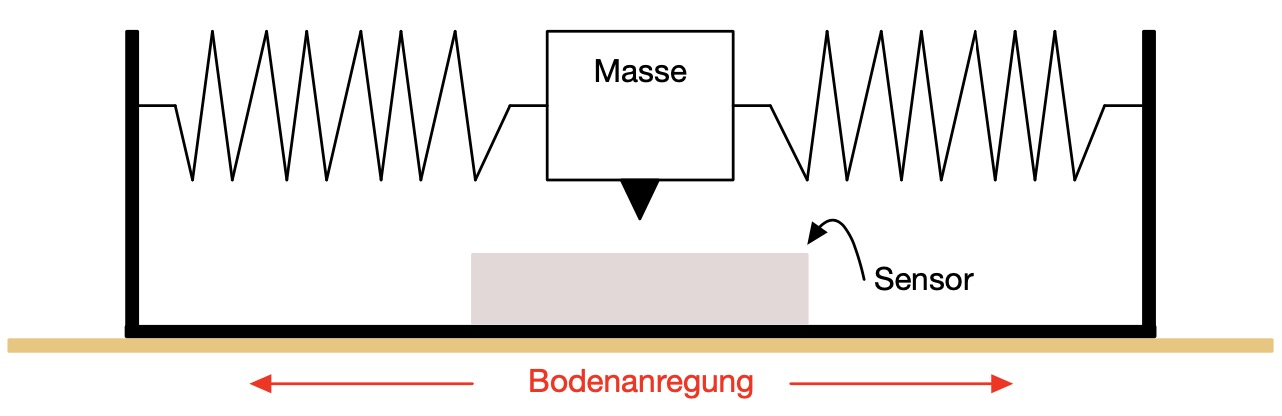
\includegraphics[width=\linewidth,keepaspectratio]{papers/erdbeben/Apperatur}
 \caption{Aufbau des Seismographen mit Gehäuse, Masse, Federn und Sensor}
 \label{erdbeben:Seismograph}
 \end{center}
\end{figure}

Unser Seismograph misst jedoch nur die Position der Masse über die Zeit. 
Wir wollen aber die Beschleunigung $a(t)$ des Boden,
respektive die Kraft,
welche auf das Gehäuse wirkt, bestimmen.  
Anhand dieser Beschleunigung,
beziehungsweise der Krafteinwirkung durch die Bodenbewegung,
wird später das Bauwerk bemessen.
Dies bedeutet, die für uns interessante Grösse $F(t)$ wird nicht durch einen Sensor erfasst. 
Jedoch können wir durch zweifaches ableiten der Positionsmessung $s(t)$ die Beschleunigung der Masse berechnen. 
Die Messung entspricht also dem zweiten Integral der Kraft $F(t)$,
wobei diese einerseits durch das Erdbeben, und andererseits durch die Federn zustande kommt.
Im Folgenden möchten wir die Erdbeben- und Federkräfte trennen.
Dafür benötigen wir zuerst eine mathematische Beschreibung unseres Systems.

\subsection{Systemgleichung}
Im Paper~\cite{erdbeben:mendezmueller} wurde das System gleich definiert und vorgegangen. 
Im Fall unseres Seismographen, handelt es sich um ein Feder-Masse-Pendel.
Dieses kann als gedämpfter harmonischer Oszillator beschrieben werden. 
Die zugehörige Differentialgleichung lautet:
\begin{equation}
	\label{erdbeben:Systemgleichung}
m\ddot s + 2k \dot s + Ds = F.
\end{equation}
wobei $m$ die Masse, $k$ die Dämpfungskonstante und $D$ die Federkonstante bezeichnet.

Für lineare Systeme ist eine Matrix-Darstellung handlicher.
Wir möchten diese Gleichung folglich in die Darstellung $\dot x = Ax$ überführen,
wobei $x$ der Zustandsvektor und $A$ die Systemmatrix bezeichnet.
Wir substituieren $\dot s = v$ für die Geschwindigkeit und erhalten das Gleichungssystem
\begin{align}
  \begin{split}
    \dot s &= v \\ 
    \dot v &= -\frac{D}{m} {s} -\frac{2k}{m} {v} + \frac{F} {m}.
  \end{split}
  \label{erdbenen:systemgleichungen}
\end{align}

Die relevanten Zustände sind also die Position $s$ und die Geschwindigkeit $v$.
Die für uns eigentlich interessante Grösse ist jedoch der Stör-Term $F$.
Dieser entspricht der Kraft durch das Erdbeben.
Deshalb nehmen wir $F$ als dritte Grösse in den Zustandsvektor auf und definieren:
\[ 
  x = \begin{pmatrix} s \\ v \\ F \end{pmatrix}
\] 
  
Für die Standard-Form $\dot x = Ax$ brauchen wir als nächstes die Ableitungen aller Elemente von $x$.
Für $s$ und $v$  haben wir diese in Gleichung~\eqref{erdbenen:systemgleichungen} bereits gefunden.
Über die Kraft $F$ wissen wir jedoch nichts.
Wir müssen also eine Annahme treffen: Die Kraft ändert sich nicht, $\dot F = 0$.
Diese Annahme ist im Allgemeinen natürlich falsch, aber etwas Besseres haben wir nicht zur Verfügung.
Wir werden dies in einem späteren Schritt kompensieren müssen.

Wir haben nun alles für die Matrix-Form von Gleichung~\eqref{erdbeben:Systemgleichung} zusammen.
Sie lautet:
\begin{equation}
  \frac{d}{dt} \begin{pmatrix} s(t) \\ v(t) \\ F(t) \end{pmatrix}
  =
 \begin{pmatrix}
  \phantom- 0 & \phantom-1& 0 \\ 
  - \frac{D}{m} &-\frac{2k}{m} & \frac{1} {m} \\
  \phantom-0 & \phantom-0 & 0\\
  \end{pmatrix}
  \begin{pmatrix} s(t) \\ v(t) \\ F(t) \end{pmatrix}.
  \label{erdbeben:systemmatrix}
\end{equation}

